

\documentclass[SPC-MASTER.tex]{subfiles}
\begin{document}
\section*{Operating Characteristic (OC) Curves}
\begin{itemize}
\item A common supplementary plot to standard quality control charts is the so-called operating characteristic or OC curve (see example below). One question that comes to mind when using standard variable or attribute charts is how sensitive is the current quality control procedure? Put in more specific terms, how likely is it that you will not find a sample (e.g., mean in an X-bar chart) outside the control limits (i.e., accept the production process as "in control"), when, in fact, it has shifted by a certain amount? 

\item This probability is usually referred to as the  (beta) error probability, that is, the probability of erroneously accepting a process (mean, mean proportion, mean rate defectives, etc.) as being "in control." 

\item Note that operating characteristic curves pertain to the false-acceptance probability using the sample-outside-of- control-limits criterion only, and not the runs tests described earlier.


\item Operating characteristic curves are extremely useful for exploring the power of our quality control procedure. The actual decision concerning sample sizes should depend not only on the cost of implementing the plan (e.g., cost per item sampled), but also on the costs resulting from not detecting quality problems. The OC curve allows the engineer to estimate the probabilities of not detecting shifts of certain sizes in the production quality.
\end{itemize}

\subsubsection*{pistonrings Data}
\begin{framed}
\begin{verbatim}
#library(qcc)
data(pistonrings); attach(pistonrings);

diameter <- qcc.groups(diameter, sample)
beta <- oc.curves.xbar(qcc(diameter, type="xbar", nsigmas=3, plot=FALSE))
print(round(beta, digits=4))

# or to identify points on the plot use
## Not run: oc.curves.xbar(qcc(diameter, 
    type="xbar", nsigmas=3, plot=FALSE), identify=TRUE)

detach(pistonrings)
\end{verbatim}
\end{framed}

\begin{figure}
\centering
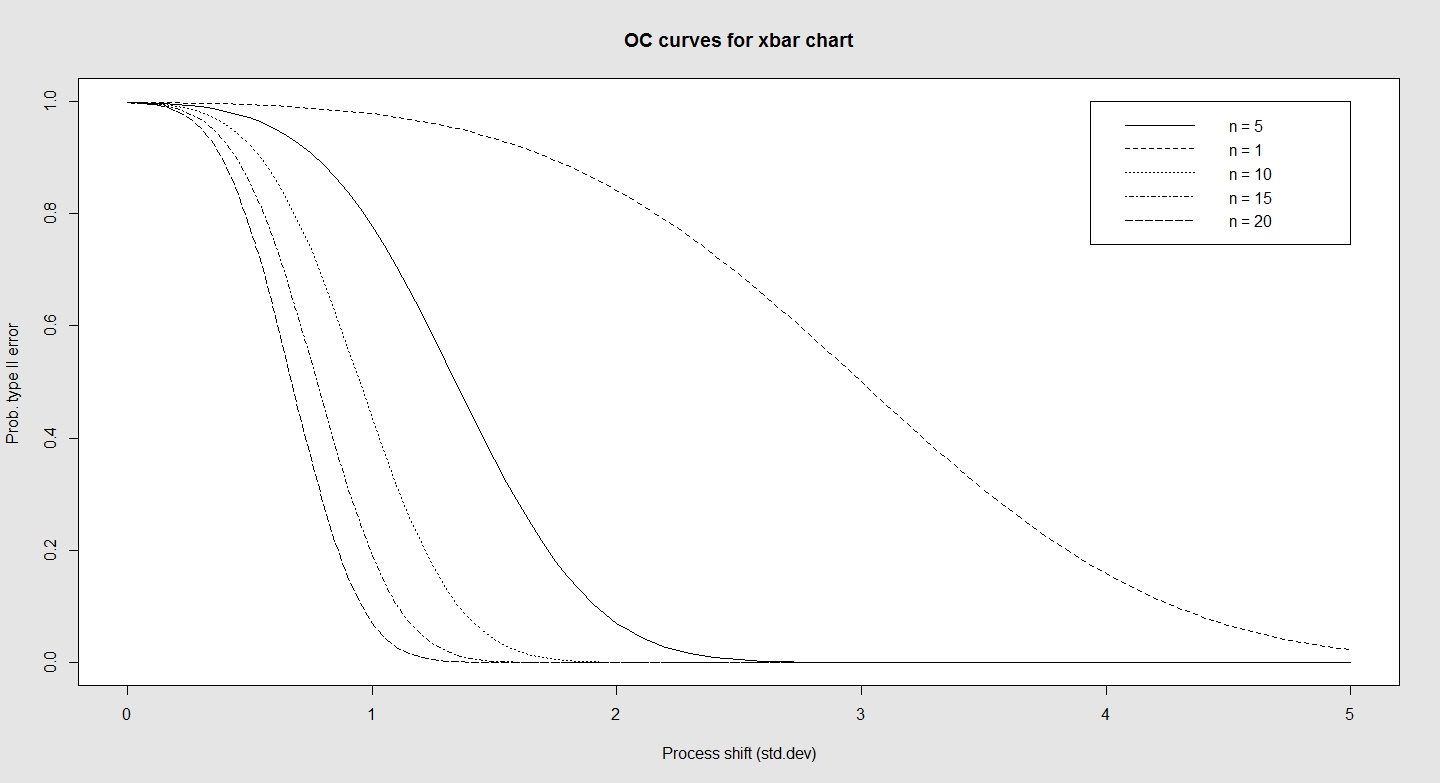
\includegraphics[width=0.7\linewidth]{images/OCpistonrings}
\caption{}
\label{fig:OCpistonrings}
\end{figure}


%%- http://support.minitab.com/en-us/minitab/17/topic-library/quality-tools/acceptance-sampling/acceptance-sampling-graphs/operating-characteristic-oc-curve/

Using an operating characteristic (OC) curve

IN THIS TOPIC
What is an operating characteristic (OC) curve?
Use an OC curve to choose an appropriate sampling plan

	What is an operating characteristic (OC) curve?
	
	The operating characteric (OC) curve depicts the discriminatory power of an acceptance sampling plan. The OC curve plots the probabilities of accepting a lot versus the fraction defective.
	
	When the OC curve is plotted, the sampling risks are obvious. You should always examine the OC curve before using a sampling plan.

	
	For example, you sample 52 rollers from a shipment of 500. If the actual \% defective is 1.5\%, you have a 0.9567 probability of accepting this lot based on the sample and a 0.0433 probability of rejecting it. If the actual \% defective is 10\%, you have a 0.0966 probability of accepting this lot and a 0.9034 probability of rejecting it.
	Examine the OC curves, AOQ curves, and ATI curves together when evaluating sampling plans.

	Use an OC curve to choose an appropriate sampling plan
	
	You can compare OC curves to help choose the appropriate sampling plan. In this case, the shift supervisor thinks sampling 52 rollers from 500 is too much. You can develop curves for various sample sizes and acceptance numbers to illustrate the increased risk.
	
	If the sample size is 35 (red line) and the \% defective is 10\%, you now have a 0.306 probability of accepting this lot.

%======================================================================================%
\end{document}
